\documentclass[12pt,a4paper,spanish]{article} 

\usepackage{graphicx} %option specific for pdfLatex compilation
\usepackage{makeidx}
\usepackage{lscape}

\usepackage[spanish]{babel}
\usepackage[utf8]{inputenc} 
\usepackage{indentfirst}

\usepackage[margin=2cm]{geometry}
\begin{document}
\begin{titlepage}
\begin{center}

% Upper part of the page. The '~' is needed because \\
% only works if a paragraph has started.

\textsc{\LARGE \textbf{Universidad de Buenos Aires}}\\%[1cm]
\vfill
\textsc{\LARGE \textbf{Introducción a los Sistemas Distribuidos}}\\%[0.5cm]
\vfill
\textsc{\LARGE \textbf{(75.43)}}\\%[0.5cm]
\vfill
% Title
%\HRule \\[0.4cm]
\vfill
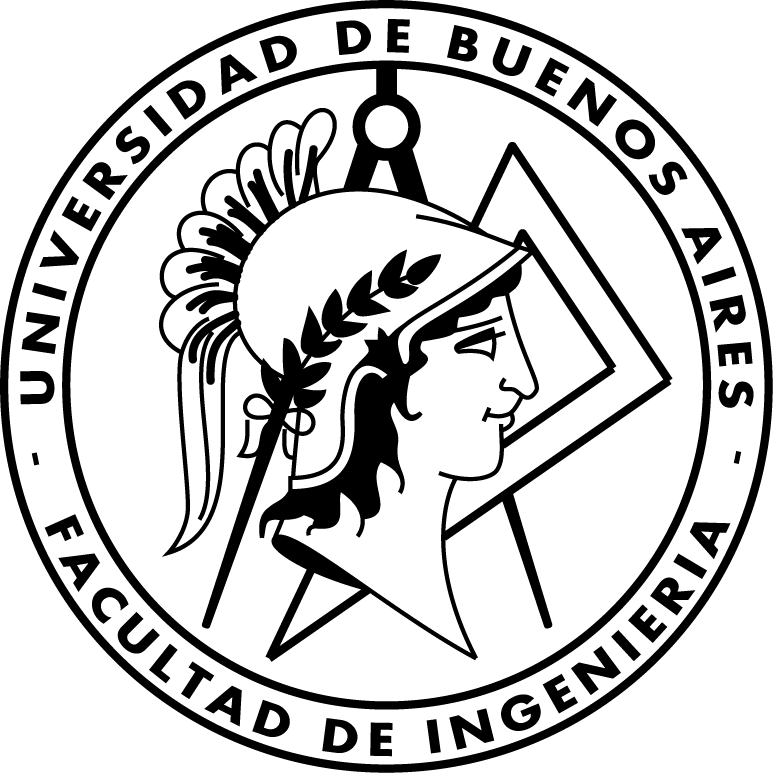
\includegraphics[scale=1.25]{./logo.png}~\\[2cm]
%\HRule \\[1.5cm]
{ \huge \bfseries Trabajo Práctico Grupal}\\%[0.25cm]
\vfill
{ \huge \bfseries Grupo 5}\\%[0.25cm]
\vfill
{\Large
\begin{tabular}{|c|c|c|}
\hline
Apellidos y nombres 		& Padrón	& 	Mail \\
\hline
Goldberg, Juan Sebastián 			& 82078		& sebas.goldberg@gmail.com \\
\hline
Lotto, Marco 				& 91967 	& marcol91@gmail.com \\
\hline
Piechotka, Federico 			& 92126 	& fpiechotka@gmail.com \\
\hline
Pérez Dittler, Ezequiel 		& 91135 	& ezeperez26@gmail.com \\
\hline
Rodriguez Genaro, Leandro 		& 92098  	& leandro.rodriguezg@gmail.com \\
\hline
\end{tabular}
}
\vfill

% Bottom of the page
{\large \today}

\end{center}
\end{titlepage}

\newpage
\tableofcontents
\newpage

\section{Subnetting}
\subsection{Asignación de direcciones IP a las redes}
\begin{tabular}{|c|c|c|c|c|c|}
	\hline
	Subred & Nombre & Hosts & Hosts máx. & Dirección & Máscara \\
	\hline
	\hline
	A &  &  &  &  &  \\
	\hline
\end{tabular}



\subsubsection{Asignación IP a routers, servers y hosts}

\begin{tabular}{|c|c|c|c|c|}
	\hline
	Subred & Dispocitivo & Interface & Dirección & Máscara \\
	\hline
	\hline
	A &  &  &  & \\
	\hline
	  & R2 &  &  &  \\
	\hline
\end{tabular}



\begin{tabular}{|c|c|c|c|c|}
	\hline
	Subred & Dispocitivo & Interface & Dirección & Máscara \\
	\hline
	\hline
	F & & & & \\
	\hline
	  &  &  &  &  \\
	\hline
\end{tabular}

\subsubsection{Asignación IP a routers en Frame Relay}

\begin{tabular}{|c|c|c|c|c|c|}
	\hline
	Subred & Dispocitivo & Interface & Dirección & Máscara & DLCI \\
	\hline	
	\hline
	 &  &  &  &  &  \\
	\hline
\end{tabular}



\subsection{Tablas de Ruteo Estático de Chos Malal}
\subsubsection{R1}
\begin{tabular}{|c|c|c|c|c|c|}
	\hline
	Red & Dirección Red & Máscara & Next Hop & Dirección Next Hop & Metrica \\
	\hline
	\hline
	A &  &  &  &  & 1\\ % R1-R3
 	  &  &  &  &  & 10 \\ % R1-R2
	\hline	
	B & & & & &\\
	\hline
\end{tabular}

\subsubsection{R2}
\begin{tabular}{|c|c|c|c|c|c|}
	\hline
	Red & Dirección Red & Máscara & Next Hop & Dirección Next Hop & Metrica \\
	\hline
	\hline
	A &  &  &  &  & 1\\
 	  &  &  &  &  & 10 \\
	\hline	
	B & & & & &\\
	\hline
\end{tabular}


\subsubsection{R3}
\begin{tabular}{|c|c|c|c|c|c|}
	\hline
	Red & Dirección Red & Máscara & Next Hop & Dirección Next Hop & Metrica \\
	\hline
	\hline
	A &  &  &  &  & 1\\
 	  &  &  &  &  & 10 \\
	\hline	
	B & & & & &\\
	\hline
\end{tabular}

\subsubsection{R4}
\begin{tabular}{|c|c|c|c|c|c|}
	\hline
	Red & Dirección Red & Máscara & Next Hop & Dirección Next Hop & Metrica \\
	\hline
	\hline
	A &  &  &  &  & 1\\
 	  &  &  &  &  & 10 \\
	\hline	
	B & & & & &\\
	\hline
\end{tabular}

\subsubsection{R5}
\begin{tabular}{|c|c|c|c|c|c|}
	\hline
	Red & Dirección Red & Máscara & Next Hop & Dirección Next Hop & Metrica \\
	\hline
	\hline
	A &  &  &  &  & 1\\
 	  &  &  &  &  & 10 \\
	\hline	
	B & & & & &\\
	\hline
\end{tabular}

\subsubsection{R6}
\begin{tabular}{|c|c|c|c|c|c|}
	\hline
	Red & Dirección Red & Máscara & Next Hop & Dirección Next Hop & Metrica \\
	\hline
	\hline
	A &  &  &  &  & 1\\
 	  &  &  &  &  & 10 \\
	\hline	
	B & & & & &\\
	\hline
\end{tabular}


\subsection{Tablas de Ruteo Estático de Aluminé}

\subsubsection{R12}
\begin{tabular}{|c|c|c|c|c|c|}
	\hline
	Red & Dirección Red & Máscara & Next Hop & Dirección Next Hop & Metrica \\
	\hline
	\hline
	A &  &  &  &  & 1\\
 	  &  &  &  &  & 10 \\
	\hline	
	B & & & & &\\
\end{tabular}

\subsubsection{R13}
\begin{tabular}{|c|c|c|c|c|c|}
	\hline
	Red & Dirección Red & Máscara & Next Hop & Dirección Next Hop & Metrica \\
	\hline
	\hline
	A &  &  &  &  & 1\\
 	  &  &  &  &  & 10 \\
	\hline	
	B & & & & &\\
	\hline
\end{tabular}

\subsubsection{R14}
\begin{tabular}{|c|c|c|c|c|c|}
	\hline
	Red & Dirección Red & Máscara & Next Hop & Dirección Next Hop & Metrica \\
	\hline
	\hline
	A &  &  &  &  & 1\\
 	  &  &  &  &  & 10 \\
	\hline	
	B & & & & &\\
	\hline
\end{tabular}

\subsubsection{R15}
\begin{tabular}{|c|c|c|c|c|c|}
	\hline
	Red & Dirección Red & Máscara & Next Hop & Dirección Next Hop & Metrica \\
	\hline
	\hline
	A &  &  &  &  & 1\\
 	  &  &  &  &  & 10 \\
	\hline	
	B & & & & &\\
	\hline
\end{tabular}

\subsubsection{R16}
\begin{tabular}{|c|c|c|c|c|c|}
	\hline
	Red & Dirección Red & Máscara & Next Hop & Dirección Next Hop & Metrica \\
	\hline
	\hline
	A &  &  &  &  & 1\\
 	  &  &  &  &  & 10 \\
	\hline	
	B & & & & &\\
	\hline
\end{tabular}

\newpage
\section{Frame Relay}
Para el armado de la red Frame Relay se usaron 6 \emph{Routers 3600}
con las siguientes configuraciones de DLCI en cada uno.
\subsection{FR1}
\begin{tabular}{|c|c|c|c|}
\hline
Interface In & DLCI In & Interface Out & DLCI Out \\
\hline
\hline
 s0/0 &  & Serial0/1 &  \\
\hline
\end{tabular}

\subsection{FR2}
\begin{tabular}{|c|c|c|c|}
\hline
Interface In & DLCI In & Interface Out & DLCI Out \\
\hline
\hline
 s0/0 &  & Serial0/1 &  \\
\hline
\end{tabular}

\subsection{FR3}
\begin{tabular}{|c|c|c|c|}
\hline
Interface In & DLCI In & Interface Out & DLCI Out \\
\hline
\hline
 s0/0 &  & Serial0/1 &  \\
\hline
\end{tabular}

\subsection{FR4}
\begin{tabular}{|c|c|c|c|}
\hline
Interface In & DLCI In & Interface Out & DLCI Out \\
\hline
\hline
 s0/0 &  & Serial0/1 &  \\
\hline
\end{tabular}

\subsection{FR5}
\begin{tabular}{|c|c|c|c|}
\hline
Interface In & DLCI In & Interface Out & DLCI Out \\
\hline
\hline
 s0/0 &  & Serial0/1 &  \\
\hline
\end{tabular}

\subsection{FR6}
\begin{tabular}{|c|c|c|c|}
\hline
Interface In & DLCI In & Interface Out & DLCI Out \\
\hline
\hline
 s0/0 &  & Serial0/1 &  \\
\hline
\end{tabular}

\newpage
\subsection{Esquema de la red Frame Relay}
%	\includegraphics[scale=0.35,angle=90]{./FR.png}~\\


\newpage
\section{Túneles GRE}
\subsection{Configuracion de los Routers}
\subsubsection{R6}
{\small
\begin{verbatim}

\end{verbatim}
}

\subsubsection{R11}
{\small
\begin{verbatim}

\end{verbatim}
}

\subsubsection{R12}
{\small
\begin{verbatim}

\end{verbatim}
}

\subsubsection{Internet}

Dentro de la topología se simuló el servicio de Internet mediante un router C3600. El objetivo de la utlización del túnel GRE fue permitir el enrutamiento de direcciones privadas entre el par de routers que se comunican a través de Internet. La configuración de los túneles GRE se basó en el apunte brindado por la cátedra. 

Se utilizaron tres direcciones públicas /30 para cada enlace ( R6-Internet, R11-Internet y R12-Internet) a partir de la dirección ip dedicada a Internet. Luego se le asignó una direccion privada /30 para el túnel que simula conectar directamente los routers R6 con R11, R6 con R12 y R11 con R12. 

Lo que finalmente se obtiene, es un encapsulamiento de un paquete IP que tiene como destino una dirección privada dentro de otro paquete IP con direccionamiento público, más la existencia de un encabezado GRE. Los routers donde se configura el túnel son los encargados de manipular estos paquetes, armandolos y desarmandolos según corresponda.

Dentro del trabajo práctico, esto se traslada a la posibilidad de que tanto los dispositivos y las redes existenes del lado de R6 como las de R11 puedan comunicarse entre sí, a pesar de que sean redes privadas con un servicio de Internet en el medio. Para esto se encapsula el destino (10.xxx.xxx.xxx) con el encabezado GRE más otro encabezado IP con direccion pública (139.67.2.xxx). Este paquete atraviesa internet, y al llegar al otro lado del túnel, el router descarta el encabezado GRE y el paquete IP con direccion pública, para posteriormente entregarlo a quien corresponda.

{\small
\begin{verbatim}

\end{verbatim}
}

\subsection{Esquema del túnel GRE}
%	\includegraphics[scale=0.50]{./GRE.png}~\\

\newpage
\section{VRRP}
\subsection{Configuración de los Routers}

\subsubsection{Sede Chos Malal}
\paragraph{R4}
{\small
\begin{verbatim}

\end{verbatim}

\paragraph{R5}
{\small
\begin{verbatim}

\end{verbatim}
}

\subsubsection{Sede Junín de los Andes}
\paragraph{R8}
{\small
\begin{verbatim}

\end{verbatim}
}

\paragraph{R9}
{\small
\begin{verbatim}

\end{verbatim}
}

\section{OSPF}
Se implementó OSPF para ruteo dinámico en la sede Junín de los Andes.

Los routers distribuyen sus rutas estáticas en las actualizaciones LS Update 
que envían.
Para evitar que envíen dicha información más allá de los límites de la sede, 
se pasivaron las interfaces correspondientes de aquellos routers en los bordes.

\subsection{Configuración de los Routers}
\subsubsection{R7}
{\small
\begin{verbatim}
!
router ospf 100
 log-adjacency-changes
 redistribute static subnets
 passive-interface Ethernet0/0
 passive-interface Ethernet0/1
 network 10.134.1.0 0.0.0.255 area 0
 network 172.13.1.192  0.0.0.3 area 0
 network 172.13.1.200  0.0.0.3 area 0
 network 10.134.13.44  0.0.0.3 area 0
!
\end{verbatim}
}

\subsubsection{R8}
{\small
\begin{verbatim}
!
router ospf 100
 log-adjacency-changes
 redistribute static
 network 10.134.1.0 0.0.0.255 area 0
 network 10.134.13.128  0.0.0.31 area 0
!
\end{verbatim}
}

\subsubsection{R9}
{\small
\begin{verbatim}
!
router ospf 100
 log-adjacency-changes
 redistribute static subnets
 passive-interface Ethernet0/2
 network 10.134.1.0 0.0.0.255 area 0
 network 10.134.13.40  0.0.0.3 area 0
 network 10.134.13.128  0.0.0.31 area 0
 network 10.134.5.128 0.0.0.127 area 0
!
\end{verbatim}
}

\subsubsection{R10}
{\small
\begin{verbatim}
!
router ospf 100
 log-adjacency-changes
 redistribute static
 network 10.134.5.128 0.0.0.127 area 0
 network 10.134.13.96  0.0.0.31 area 0
!
\end{verbatim}
}

\subsubsection{R11}
{\small
\begin{verbatim}
!
router ospf 100
 log-adjacency-changes
 redistribute static subnets
 passive-interface Tunnel10
 passive-interface Tunnel20
 passive-interface Ethernet0/1
 network 10.134.5.128 0.0.0.127 area 0
 network 10.134.13.36  0.0.0.3 area 0
 network 10.134.13.28  0.0.0.3 area 0
!
\end{verbatim}
}

\newpage
\section{DNS}
Para obtener la ip asociado a un nombre(o viceversa), cada host realiza la solicitud a su servidor DNS local, que corresponde a la zona en la que se encuentre. En la sede Chos Malal se corresponde el DNS 1 y para Junín de los Andes y Alumine corresponde el DNS 2. Cuando un servidor DNS no conoce un nombre de dominio y posee el mismo dominio de la empresa, este realiza una solicitud al DNS root que le responde con la dirección del otro servidor DNS para así consultar por la respuesta de la solicitud inicial, y esta manera se resolvería la solicitud de forma iterativa.

Para la resolución de nombres de dominio y distinguir los diferentes hosts pertenecientes a cada sede, se agregaron dominios con el nombre de la sede al dominio que ya posee la empresa (neuquen.dc.fi.uba.ar). Un ejemplo podría seria, para el host A que se encuentra en al Red C (denominada como Concorde) perteneciente a la sede Chos Malal, su dominio asociado seria a.chosmalal.neuquen.dc.fi.uba.ar. Otro ejemplo podría ser del servidor FTP, que se encuentra en la red B (denominada como Boeing) en la sede Alumine con el nombre asociado de ftp.alumine.neuquen.dc.fi.uba.ar.

\section{OPEN VPN}
Se crearon 7 VPNs, una para cada red conectada a dispositivos físicos.
\subsection{Servers}
Los 7 VPN servers corren en paralelo en 7 puertos diferentes, en la misma PC que tiene la topología.
Para cada uno, está configurada una interfaz tap en modo promiscuo, la cual escucha todos los paquetes que llegan.
A través de NIO ethernet, se encuentran conectadas dichas interfaces a la LAN de la topología correspondiente.
\subsection{Clientes}
Para cada cliente, se encuentra su archivo de configuración con la IP y puerto del servidor correspondiente, además de su certificado
y otros parámetros.
Al conectarse a una VPN, existe un script que configura la conexión y las rutas del dispositivo (i.e. su default gateway).

\newpage
\section{Anexo}
\subsection{Topología}
%\begin{figure}[h!]
%  \centering
%	\includegraphics[scale=0.65,angle=90]{./Topologia.png}~\\
\subsection{Topología con redes marcadas}
%\begin{figure}[h!]
%  \centering
%	\includegraphics[scale=0.65,angle=90]{./TopologiaMarcada.png}~\\

\subsection{Esquema de la topología}
%	\includegraphics[scale=0.35,angle=90]{./TopologiaEsquema.png}~\\
%\end{figure}


\end{document}
